\chapter{Architecture}
\label{chp:architecture} 

The purpose of this thesis is to build an end to end system, to be able to transfer data all the way from a sensor connected to a microcontroller to a server. This chapter will describe in detail how the different components of the system has been connected together, and how the different protocols has been configured to read and transfer data efficiently. 


\begin{figure}[ht]
    \centering
    \includegraphics[scale=0.7]{MasterArchitecture.png}    \caption{System architecture}
    \label{fig:systemArchitecture}
\end{figure}

\newpage

There are two main limitations in a network such as this:

\begin{itemize}
  \item Computational power in the different nodes 
  \item Network limitations between the nodes
\end{itemize}

A central part of the testing in this thesis will be to test the different limitations, and to understand the pros and cons of doing computations in end nodes, compared to transferring information to a server with \textit{much} more computational power. Power usage is very often closely related to computational power, and will also be a central factor. The next section will contain a walk through of the system, from the smallest to the biggest component, to explain their computational and power capabilities, and how they can communicate efficiently. 

%Computational power is closely related to power usage. The nRF52 microcontroller is battery powered using a small \textit{3V Lithium CR 2032} battery. Given this limitation the computational power will be limited as well. The optimal solutions therefore seems to handle as little data as possible here. 


%Figure \ref{fig:systemArchitecture} shows how the complete End-to-End system of this thesis is set up. In short terms, the \textit{ADXL345 Accelerometer} is connected to a \textit{Nordic Semiconductor nRF52} using the \gls{i2c} interface. This requires four cables (noted from nRF52 to ADXL345): 

\section{Connecting nRF52 and ADXL345}

The ADXL345 Accelerometer used was connected using \gls{i2c}, which is quite straight forward using the nRF52. Connection scheme is as follows (nRF52 -> ADXL345): 

\begin{itemize}
  \item 5V -- VIN		\tab  	\textit{Power source, GREEN in Figure\ref{fig:nrf-adxl345}}
  \item GND -- GND 		\tab 	\textit{Ground, RED in Figure \ref{fig:nrf-adxl345}}
  \item P0.27 -- SDA	\tab	\textit{\gls{i2c} Serial Data Line}
  \item P0.26 -- SCL	\tab 	\textit{\gls{i2c} Serial Clock Line}
\end{itemize} 

\begin{figure}[ht]
    \centering
    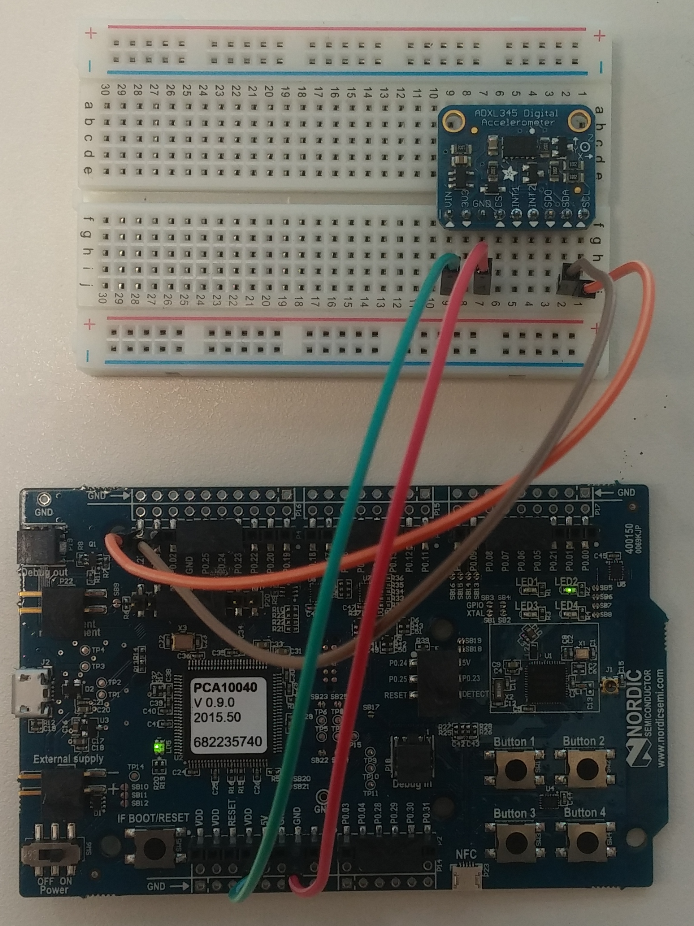
\includegraphics[scale=0.35]{nrf-adxl.png}    \caption{Connected nRF52 -- ADXL345}
    \label{fig:nrf-adxl345}
\end{figure}

After this is done it is possible to write to and read from the registers of the accelerometer over the two SDA and SCL cables. 

\begin{figure}[h]
    \centering
    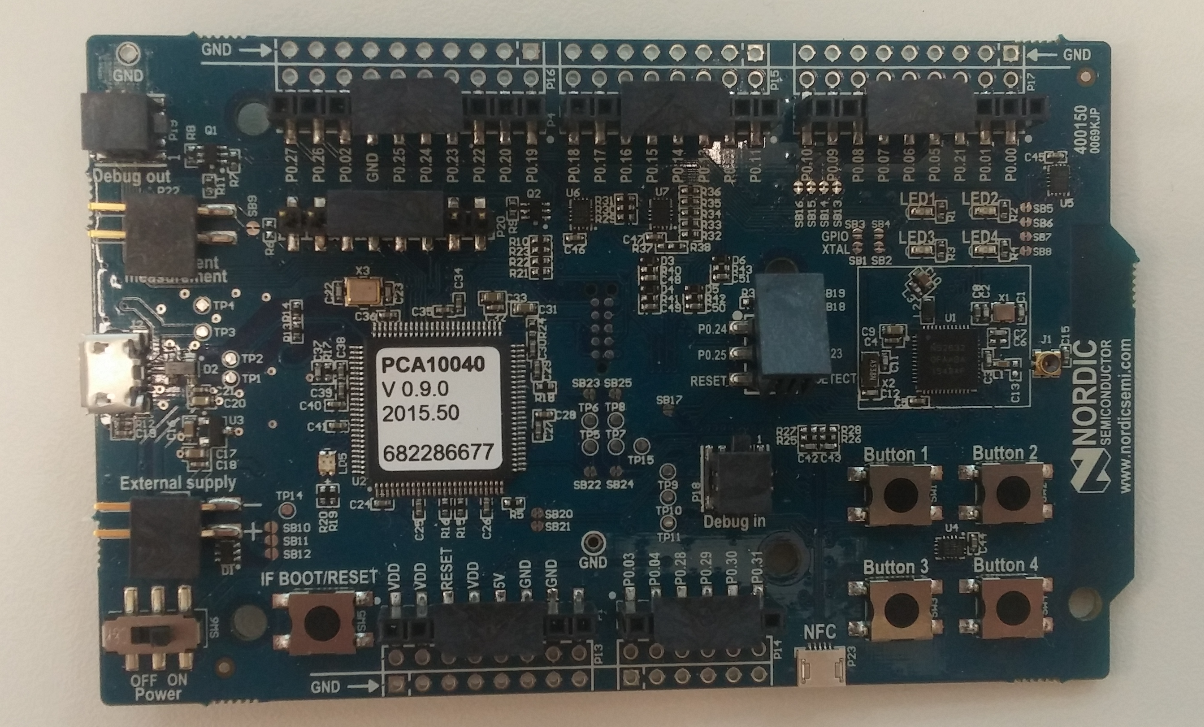
\includegraphics[scale=0.32]{nrf52.png}    \caption{Nordic Semiconductor NRF52}
    \label{fig:nrf52picture}
\end{figure}

The communication between the nRF52 in Figure \ref{fig:nrf52picture} and the Raspberry Pi in Figure \ref{fig:piPicture}, is done using \gls{6lowpan} over \gls{ble}. 

\begin{figure}[h]
    \centering
    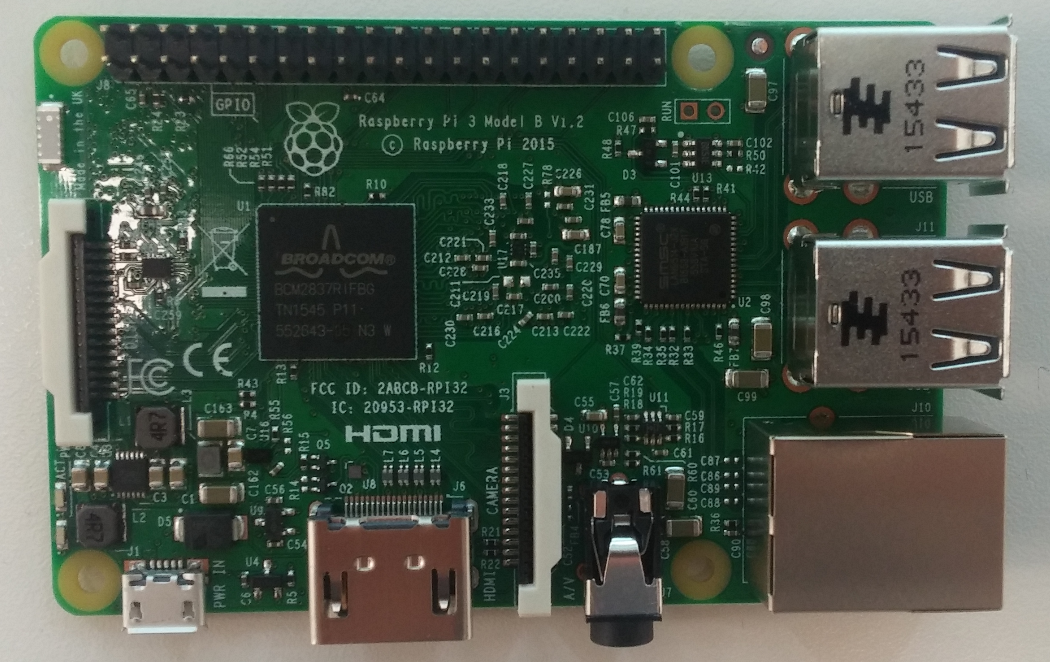
\includegraphics[scale=0.35]{pi3.png}    \caption{Raspberry Pi 3}
    \label{fig:piPicture}
\end{figure}




\section{\gls{6lowpan} and \gls{ble}}



\section{Connecting Raspberry Pi and nRF52}



As a microcontroller the nRF52 works great, both as a low-power and powerful device. 

To set up the communication between these two, the two code examples TWI and Observable server from Nordic Semiconductor was used as a starting point. It was however quite tricky to set connect these two together the first time. The following recipe is what worked best. 

Install an \gls{os} on the Raspberry Pi that has a Linux kernel version later than 3.18. On \textit{Raspbian} version 3.18 is the only stable (Note: Feb. 2016), but \textit{Ubuntu Mate} is stable in version 4.15. \textit{Ubuntu Mate} was therefore chosen as the best and most stable \gls{os}. When this is done a resizing of the file system is needed to use all the capacity of the memory card. 

To use \gls{ble}, install Bluez and radvd using \textit{apt-get}:

\begin{lstlisting}
apt-get install radvd wireshark bluez
apt-get upgrade
apt-get update
\end{lstlisting}

To activate \gls{ipv6} forwarding, uncomment the following line in \textit{etc/sysctl.conf}

\begin{verbatim}
net.ipv6.conf.all.forwarding=1
\end{verbatim}

Add the \textit{bt0 interface} in \textit{radvd.conf}:

\begin{verbatim}
touch /etc/radvd.conf
pico /etc/radvd.conf

# Write in

interface bt0
{
    AdvSendAdvert on;
    prefix 2001::/64
    {
        AdvOnLink off;
        AdvAutonomous on;
        AdvRouterAddr on;
    };
};
\end{verbatim} 

To mount the modules \textit{bluetooth\_6lowpan, 6lowpan and radvd}, add the following to \textit{/etc/modules}. 

\begin{verbatim}
bluetooth_6lowpan
6lowpan
radvd
\end{verbatim}

It is now possible to use the \textit{hcitool} command. 

\begin{verbatim}
hcitool lescan
\end{verbatim}

This command will scan for \gls{ble} devices nearby, and find the bluetooth address, for instance \textit{0211:22FF:FE33:4455}. To connect, run the following: 

\begin{verbatim}
echo 1 > /sys/kernel/debug/bluetooth/6lowpan_enable
echo "connect 0211:22FF:FE33:4455 1" > /sys/kernel/debug/bluetooth/6lowpan_control
service radvd restart
\end{verbatim}

The command \textit{hcitool con} shows the connected \gls{ble} devices. If the device is connected, the connection can be tested by typing

\begin{verbatim}
ping6 2001::0211:22FF:FE33:4455
\end{verbatim}





As mentioned before, using the basic example of the observable server it was easy to send \gls{coap} messages without the need of an \gls{ack} for every message. 
 

\subsection{\gls{spi}}



\subsection{\gls{i2c}}


\subsection{Problems}




